\documentclass[../TDE4-E5.tex]{subfiles}%

\begin{document}
\section[s]"1"{Étude énergétique d'un oscillateur harmonique électrique}

\enonce{%
	\noindent
	\begin{minipage}{0.6\linewidth}
		Dans le circuit ci-contre, la source idéale de courant est brusquement
		éteinte. On le modélise par un échelon de courant, $\eta(t)$ passant de
		$I_0$ à 0 à l'instant $t = 0$. On appelle $\Ec_{\rm tot} = \Ec_C + \Ec_L$
		l'énergie électrique totale stockée dans le condensateur et la bobine.
	\end{minipage}
	\begin{minipage}{0.4\linewidth}
		\centering
		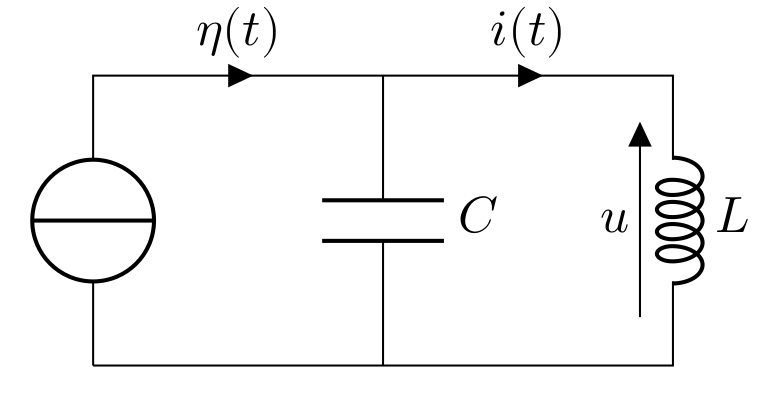
\includegraphics[width=\linewidth]{lc_energie}
	\end{minipage}
}%

\QR{%
	Exprimer $\DS \dv{\Ec_{\rm tot}}{t}$ en fonction de $i$ et $\DS
		\dv{i}{t}$.
}{%
	Une fois le générateur de courant stoppé, l'énergie totale est la somme de
	l'énergie stockée dans le condensateur et de celle stockée dans la bobine,
	soit
	\[\Ec_{\rm tot} = \frac{1}{2}Cu^2 + \frac{1}{2}Li^2\]
	En dérivant on a donc
	\[ \dv{\Ec_{\rm tot}}{t} = \frac{1}{2}C\times 2u \dv{u}{t} +
		\frac{1}{2}\times 2i \dv{i}{t}\]
	Comme on demande de ne faire apparaître que $i$ dans le résultat, on
	remplace $u$ avec la relation courant-tension de la bobine et on développe~:
	\begin{align*}
		\dv{\Ec_{\rm tot}}{t}         & = \frac{1}{2}C \times 2L \dv{i}{t} \dv{}{t} \left(
		L \dv{i}{t}\right) + \frac{1}{2} L\times 2i \dv{i}{t}                              \\
		\Leftrightarrow
		\dv{\Ec_{\rm tot}}{t}         & = L^2C \dv{i}{t} \dv[2]{i}{t} + Li \dv{i}{t}       \\
		\Leftrightarrow
		\Aboxed{\dv{\Ec_{\rm tot}}{t} & = L \dv{i}{t} \left( LC \dv[2]{i}{t} + i
			\right)}
	\end{align*}
}%

\QR{%
	Justifier qualitativement que $\Ec_{\rm tot}$ est constante. En
	déduire l'équation différentielle vérifiée par $i$.
}{%
	Le circuit ne compte qu'une bobine et un condensateur qui stockent de
	l'énergie sans la dissiper, et donc aucune résistance. L'énergie électrique
	dans le circuit est donc constante, et on en déduit qu'$\forall t \in
		\Rb^+$~:
	\begin{equation*}
		\dv{\Ec_{\rm tot}}{t} = 0
		\qdonc
		L \dv{i}{t} \left( LC \dv[2]{i}{t} + i \right) = 0
	\end{equation*}
	On a donc un produit qui est nul. Or, la tension de la bobine $L \dv{i}{t}$
	ne peut être constamment nulle, c'est donc le terme entre parenthèses qui
	est nul, c'est-à-dire~:
	\begin{equation*}
		LC \dv[2]{i}{t} + i = 0
		\Longleftrightarrow
		\boxed{ \dv[2]{i}{t} + \w_0{}^2i = 0} \qavec \boxed{\w_0 =
			\frac{1}{\sqrt{LC}}}
	\end{equation*}
}%

\QR{%
	Retrouver cette équation par application des lois des nœuds et des
	mailles.
}{%
	$C$ et $L$ sont en parallèle, donc partagent la même tension $u$. Soit $i_C$
	le courant traversant $C$. Comme $\eta(t\geq0) = 0$, la loi des nœuds donne
	\[0 = i_C + i\qdonc C\dv{u}{t} + i = 0\]
	avec la RCT du condensateur. Comme $u$ est aussi la tension de $L$, avec la
	RCT de la bobine on retrouve bien
	\begin{equation*}
		\boxed{LC \dv[2]{i}{t} + i = 0}
	\end{equation*}
}%

\QR{%
	Établir les conditions initiales sur $i$ et sa dérivée.
}{%
	À $t=0^-$, le circuit est alimenté par $\eta = I_0$ et on suppose le régime
	permanent atteint~: la bobine est donc équivalente à un fil, et le
	condensateur à un interrupteur ouvert. On en déduit donc
	\[i(0^-) = I_0 \qet u(0^-) = 0\]
	Par continuité de $i$ traversant la bobine et de $u$ aux bornes du
	condensateur, on a
	\[ \boxed{i(0^-) = i(0^+) = I_0} \qet u(0^-) = u(0^+) = 0\]
	Or, $u(0^+) = L \dv{i}{t} (0^+)$ d'après la RCT de la bobine. La seconde
	condition initiale est donc
	\[ \boxed{ \qty(\dv{i}{t})_{0^+} = 0}\]
}%

\QR{%
	En déduire l'expression de $i(t)$.
}{%
	L'équation étant homogène, la solution générale s'écrit
	\[ i(t) = A\cos(\w_0t) + B\sin(\w_0t)\]
	Avec la première CI, on a
	\[ i(0) = I_0 = A\]
	et avec la seconde on a
	\begin{gather*}
		\dv{i}{t} = -A\w_0\sin(\w_0t) + B\w_0\cos(\w_0t)\\
		\Rightarrow
		\qty(\dv{i}{t})_{0} = \w_0B = 0\qdonc B = 0
	\end{gather*}
	Finalement, on trouve sans surprise
	\begin{equation*}
		\boxed{i(t) = I_0\cos(\w_0t)}
	\end{equation*}
}%

\end{document}
